%\documentclass{article}
\documentclass[a4paper,12pt]{article}
% Seitenränder in schön für Steven
\usepackage[paper=a4paper,left=25mm,right=25mm,top=25mm,bottom=25mm]{geometry}
\usepackage{enumitem}
\usepackage{amsmath}
\usepackage{float}
\usepackage{graphicx}
\usepackage{tikz}
\usepackage{titling}

\floatstyle{boxed}
\restylefloat{figure}

% Schusterjungen und Hurenkinder bestrafen
\clubpenalty50000
\widowpenalty50000
\displaywidowpenalty=50000

% Buchstaben mit kringel drum: %
\newcommand*\mycirc[1]{%
	\begin{tikzpicture}[baseline=(C.base)]
	\node[draw,circle,inner sep=1pt](C) {#1};
	\end{tikzpicture}}

\author{Benedict Hans, Christoph Dollase, Steven Te\ss endorf}
\setlength{\droptitle}{-5em} % set the title to the top of the page

% ==========================
% ===== START HERE!! =======
% ==========================
\title{ \textbf{Problem Sheet 5}} % Nummer des Aufgabenblattes
\setcounter{section}{5} % Nummer des Aufgabenblattes

\begin{document}	 
	\maketitle	 %Some Vodoo-magic
	
\subsection{Data Encoding}
\textbf{The following bit sequence shall be encoded: 0101110010 \\
	Represent the sequence in a time-voltage-diagram using the following encoding schemes: Non-Return-to-Zero (NRZ), Return-to-Zero (RZ), Differential-Non-Return-to-Zero, Manchester, Differential-Manchester}
	
\begin{figure}[H]
	\centering
	\begin{tikzpicture}
		%Basis: grid, Achsen, Beschriftung
		\draw[lightgray] (0,-1.5) grid [xstep=1cm,ystep=1cm] (10,1.5); %some help grid lines for orientation 
		\draw[thick, ->] (0,0) -- (11,0);
		\draw[thick, <->] (0,-1.5) -- (0,1.5);
		\node [right] at (11,0) {$t$};
		\node [align=center,above] at (0,1.5) {signal amplitude \\ (in Volt)};
		\node [left] at (0,1) {+5};
		\node [left] at (0,-1) {-5};
		% egentliche Pfad für den Code:
		% 00 01 10 11 00 11 10 01 10 10
		% Codierung in Volt:
		% -2 -1  1  2 -2  2  1 -1  1  1
		\draw[line width=2pt, red] (0,-1) -- (0.5,-1) -- (0.5,0) -- (1,0) -- (1,1) -- (1.5,1) -- (1.5,0) -- (2,0) -- (2,-1) -- (2.5,-1) --  (2.5,0) -- (3,0) -- (3,1) -- (3.5,1) -- (3.5,0) -- (4,0) -- (4,1) -- (4.5,1) -- (4.5,0)-- (5,0) -- (5,1) -- (5.5,1) -- (5.5,0) -- (6,0) -- (6,-1) -- (6.5,-1) -- (6.5,0) -- (7,0) -- (7,-1) -- (7.5,-1) -- (7.5,0) -- (8,0) -- (8,1) -- (8.5,1) -- (8.5,0) -- (9,0) -- (9,-1) -- (9.5,-1) -- (9.5,0) -- (10,0) ;
		% Legende aufzählung der bits:
		\node [align=center, below left] at (0,-1.5) {code};
		\node [align=center,below] at (0.5,-1.5)
			{\textcolor{blue}{$[0]$}};
		\node [align=center,below] at (1.5,-1.5)
			{\textcolor{blue}{$[1]$}};
		\node [align=center,below] at (2.5,-1.5)
			{\textcolor{blue}{$[0]$}};
		\node [align=center,below] at (3.5,-1.5)
			{\textcolor{blue}{$[1]$} };
		\node [align=center,below] at (4.5,-1.5)
			{\textcolor{blue}{$[1]$} };
		\node [align=center,below] at (5.5,-1.5)
			{\textcolor{blue}{$[1]$} };
		\node [align=center,below] at (6.5,-1.5)
			{\textcolor{blue}{$[0]$} };
		\node [align=center,below] at (7.5,-1.5)
			{\textcolor{blue}{$[0]$} };
		\node [align=center,below] at (8.5,-1.5)
			{\textcolor{blue}{$[1]$} };
		\node [align=center,below] at (9.5,-1.5)
			{\textcolor{blue}{$[0]$} };
	\end{tikzpicture}
	\caption{Return-To-Zero diagram for bit sequence \textcolor{blue}{$[0101110010]$}.}
	\label{fig:RTZ}
\end{figure}

\begin{figure}[H]
	\centering
	\begin{tikzpicture}
	%Basis: grid, Achsen, Beschriftung
	\draw[lightgray] (0,-1.5) grid [xstep=1cm,ystep=1cm] (10,1.5); %some help grid lines for orientation 
	\draw[thick, ->] (0,0) -- (11,0);
	\draw[thick, <->] (0,-1.5) -- (0,1.5);
	\node [right] at (11,0) {$t$};
	\node [align=center,above] at (0,1.5) {signal amplitude \\ (in Volt)};
	\node [left] at (0,1) {+5};
	\node [left] at (0,-1) {-5};
	% egentliche Pfad für den Code:
	% 00 01 10 11 00 11 10 01 10 10
	% Codierung in Volt:
	% -2 -1  1  2 -2  2  1 -1  1  1
	\draw[line width=2pt, red] (0,-1) -- (1,-1) -- (1,1) -- (2,1) -- (2,-1) -- (3,-1) -- (3,1) -- (6,1) -- (6,-1) -- (8,-1) -- (8,1) -- (9,1) -- (9,-1) -- (10,-1) ;
	% Legende aufzählung der bits:
	\node [align=center, below left] at (0,-1.5) {code};
	\node [align=center,below] at (0.5,-1.5)
	{\textcolor{blue}{$[0]$}};
	\node [align=center,below] at (1.5,-1.5)
	{\textcolor{blue}{$[1]$}};
	\node [align=center,below] at (2.5,-1.5)
	{\textcolor{blue}{$[0]$}};
	\node [align=center,below] at (3.5,-1.5)
	{\textcolor{blue}{$[1]$} };
	\node [align=center,below] at (4.5,-1.5)
	{\textcolor{blue}{$[1]$} };
	\node [align=center,below] at (5.5,-1.5)
	{\textcolor{blue}{$[1]$} };
	\node [align=center,below] at (6.5,-1.5)
	{\textcolor{blue}{$[0]$} };
	\node [align=center,below] at (7.5,-1.5)
	{\textcolor{blue}{$[0]$} };
	\node [align=center,below] at (8.5,-1.5)
	{\textcolor{blue}{$[1]$} };
	\node [align=center,below] at (9.5,-1.5)
	{\textcolor{blue}{$[0]$} };
	\end{tikzpicture}
	\caption{Non-Return-To-Zero diagram for bit sequence \textcolor{blue}{$[0101110010]$}.}
	\label{fig:NRZ}
\end{figure}

\begin{figure}[H]
	\centering
	\begin{tikzpicture}
	%Basis: grid, Achsen, Beschriftung
	\draw[lightgray] (0,-1.5) grid [xstep=1cm,ystep=1cm] (10,1.5); %some help grid lines for orientation 
	\draw[thick, ->] (0,0) -- (11,0);
	\draw[thick, <->] (0,-1.5) -- (0,1.5);
	\node [right] at (11,0) {$t$};
	\node [align=center,above] at (0,1.5) {signal amplitude \\ (in Volt)};
	\node [left] at (0,1) {+5};
	\node [left] at (0,-1) {-5};
	% egentliche Pfad für den Code:
	% 00 01 10 11 00 11 10 01 10 10
	% Codierung in Volt:
	% -2 -1  1  2 -2  2  1 -1  1  1
	\draw[line width=2pt, red] (0,-1) -- (1,-1) -- (1,1) -- (3,1) -- (3,-1) -- (4,-1) -- (4,1) -- (5,1) -- (5,-1) -- (8,-1) -- (8,1) -- (10,1);
	% Legende aufzählung der bits:
	\node [align=center, below left] at (0,-1.5) {code};
	\node [align=center,below] at (0.5,-1.5)
	{\textcolor{blue}{$[0]$}};
	\node [align=center,below] at (1.5,-1.5)
	{\textcolor{blue}{$[1]$}};
	\node [align=center,below] at (2.5,-1.5)
	{\textcolor{blue}{$[0]$}};
	\node [align=center,below] at (3.5,-1.5)
	{\textcolor{blue}{$[1]$} };
	\node [align=center,below] at (4.5,-1.5)
	{\textcolor{blue}{$[1]$} };
	\node [align=center,below] at (5.5,-1.5)
	{\textcolor{blue}{$[1]$} };
	\node [align=center,below] at (6.5,-1.5)
	{\textcolor{blue}{$[0]$} };
	\node [align=center,below] at (7.5,-1.5)
	{\textcolor{blue}{$[0]$} };
	\node [align=center,below] at (8.5,-1.5)
	{\textcolor{blue}{$[1]$} };
	\node [align=center,below] at (9.5,-1.5)
	{\textcolor{blue}{$[0]$} };
	\end{tikzpicture}
	\caption{Differential-NRZ diagram for bit sequence \textcolor{blue}{$[0101110010]$}.}
	\label{fig:diffNRZ}
\end{figure}

\begin{figure}[H]
	\centering
	\begin{tikzpicture}
	%Basis: grid, Achsen, Beschriftung
	\draw[lightgray] (0,-1.5) grid [xstep=1cm,ystep=1cm] (10,1.5); %some help grid lines for orientation 
	\draw[thick, ->] (0,0) -- (11,0);
	\draw[thick, <->] (0,-1.5) -- (0,1.5);
	\node [right] at (11,0) {$t$};
	\node [align=center,above] at (0,1.5) {signal amplitude \\ (in Volt)};
	\node [left] at (0,1) {+5};
	\node [left] at (0,-1) {-5};
	% egentliche Pfad für den Code:
	% 00 01 10 11 00 11 10 01 10 10
	% Codierung in Volt:
	% -2 -1  1  2 -2  2  1 -1  1  1
	\draw[line width=2pt, red] (0,1) -- (0.5,1) -- (0.5,-1) -- (1,-1) -- (1.5,-1) -- (1.5,1) -- (2.5,1) -- (2.5,-1) -- (3.5,-1) -- (3.5,1) -- (4,1) --(4,-1) -- (4.5,-1) -- (4.5,1)-- (5,1) -- (5,-1) -- (5.5,-1) -- (5.5,1) -- (6.5,1) --  (6.5,-1) -- (7,-1) -- (7,1) -- (7.5,1) -- (7.5,-1) -- (8.5,-1) -- (8.5,1) -- (9.5,1) -- (9.5,-1) -- (9.5,-1) -- (10,-1) ;
	% Legende aufzählung der bits:
	\node [align=center, below left] at (0,-1.5) {code};
	\node [align=center,below] at (0.5,-1.5)
	{\textcolor{blue}{$[0]$}};
	\node [align=center,below] at (1.5,-1.5)
	{\textcolor{blue}{$[1]$}};
	\node [align=center,below] at (2.5,-1.5)
	{\textcolor{blue}{$[0]$}};
	\node [align=center,below] at (3.5,-1.5)
	{\textcolor{blue}{$[1]$} };
	\node [align=center,below] at (4.5,-1.5)
	{\textcolor{blue}{$[1]$} };
	\node [align=center,below] at (5.5,-1.5)
	{\textcolor{blue}{$[1]$} };
	\node [align=center,below] at (6.5,-1.5)
	{\textcolor{blue}{$[0]$} };
	\node [align=center,below] at (7.5,-1.5)
	{\textcolor{blue}{$[0]$} };
	\node [align=center,below] at (8.5,-1.5)
	{\textcolor{blue}{$[1]$} };
	\node [align=center,below] at (9.5,-1.5)
	{\textcolor{blue}{$[0]$} };
	\end{tikzpicture}
	\caption{Manchester diagram for bit sequence \textcolor{blue}{$[0101110010]$}.}
	\label{fig:manchester}
\end{figure}

\begin{figure}[H]
	\centering
	\begin{tikzpicture}
	%Basis: grid, Achsen, Beschriftung
	\draw[lightgray] (0,-1.5) grid [xstep=1cm,ystep=1cm] (10,1.5); %some help grid lines for orientation 
	\draw[thick, ->] (0,0) -- (11,0);
	\draw[thick, <->] (0,-1.5) -- (0,1.5);
	\node [right] at (11,0) {$t$};
	\node [align=center,above] at (0,1.5) {signal amplitude \\ (in Volt)};
	\node [left] at (0,1) {+5};
	\node [left] at (0,-1) {-5};
	% egentliche Pfad für den Code:
	% 00 01 10 11 00 11 10 01 10 10
	% Codierung in Volt:
	% -2 -1  1  2 -2  2  1 -1  1  1
	\draw[line width=2pt, red] (0,1) -- (0.5,1) -- (0.5,-1) -- (1,-1) -- (1.5,-1) -- (1.5,1) -- (2,1) -- (2,-1) -- (2.5,-1) -- (2.5,1) -- (3.5,1) -- (3.5,-1) -- (4.5,-1) -- (4.5,1 )-- (5.5,1) -- (5.5,-1) -- (6,-1) -- (6,1) -- (6.5,1) --  (6.5,-1) -- (7,-1) -- (7,1) -- (7.5,1) -- (7.5,-1) -- (8.5,-1) -- (8.5,1) -- (9,1) -- (9,-1) -- (9.5,-1) -- (9.5,1) -- (10,1) ;
	% Legende aufzählung der bits:
	\node [align=center, below left] at (0,-1.5) {code};
	\node [align=center,below] at (0.5,-1.5)
	{\textcolor{blue}{$[0]$}};
	\node [align=center,below] at (1.5,-1.5)
	{\textcolor{blue}{$[1]$}};
	\node [align=center,below] at (2.5,-1.5)
	{\textcolor{blue}{$[0]$}};
	\node [align=center,below] at (3.5,-1.5)
	{\textcolor{blue}{$[1]$} };
	\node [align=center,below] at (4.5,-1.5)
	{\textcolor{blue}{$[1]$} };
	\node [align=center,below] at (5.5,-1.5)
	{\textcolor{blue}{$[1]$} };
	\node [align=center,below] at (6.5,-1.5)
	{\textcolor{blue}{$[0]$} };
	\node [align=center,below] at (7.5,-1.5)
	{\textcolor{blue}{$[0]$} };
	\node [align=center,below] at (8.5,-1.5)
	{\textcolor{blue}{$[1]$} };
	\node [align=center,below] at (9.5,-1.5)
	{\textcolor{blue}{$[0]$} };
	\end{tikzpicture}
	\caption{Differential Manchester diagram for bit sequence \textcolor{blue}{$[0101110010]$}.}
	\label{fig:diffMan}
\end{figure}

\subsection{Noise and Attenuation}
\textbf{Every signal is subjected to noise.  Can you specify what noise is and how it affects the signal? Name sources of noise.  What is attenuation and how does it influence a signal?}\\
\\
Noise is an unwanted effect influencing and modificating the signal during transmission, converison or processing. In most cases the source of noice is unknown. Sources of noise:
\begin{itemize}[itemsep=0pt]
	\item Thermal noise
	\item Intermodulation
	\item noise
	\item Crosstalk
	\item Impulse noise
    \item \textcolor{red}{Quantization Noise}
\end{itemize}
\\
Attenuation is a feature of the medium where the signal is transfered and defines how much of the signal absorbed by the medium. So Attenuation affects the strength of the signal.

\pagebreak
\subsection{(Differential) Manchester}
\textbf{Consider you have measured the following signal \textit{(see assignment sheet)}.\\
The vertical lines represent the end of a bit.  Specify the bit sequence that is encoded in the signal considering that it was encoded with: Manchester baseband encoding and Differential Manchester. Can the bit sequences be specified unambiguously?}

\begin{enumerate}[itemsep=0pt]
	\item Manchester baseband encoding (also called biphase-level)
	\begin{itemize}
		\item \textcolor{blue}{$[0001011000]$}
	\end{itemize}
	\item Differential Manchester
	\begin{itemize}
		\item \textcolor{blue}{$[0001101111]$}
	\end{itemize}
\end{enumerate}
\\
As you can see above there are some constellations where (1) and (2) encode the same bits, for example the first 4 bits.
\\
\textcolor{red}{We cannot say for sure if the first bit is a zero in Differential Manchestter}
	
\subsection{Wireless Transmission}
\textbf{Consider the electromagnetic spectrum presented in the lecture slides. If you had to transmit signals  with  a  given  bandwidth, an appropriate frequency band has to be found. Frequency bands are subject to legal regulation, and also they have distinct physical properties. As a result, signals have to reside within a single frequency band and cannot be spread over several bands.}\\
\\
\textbf{Say you need to transmit a signal of 20 MHz bandwidth. Can you send it in the electromagnetic base band?}\\
\\
yes, there are several bands available in the electromagnetic base band to transmit a 20MHz signal\\
\textcolor{red} {It is not possible in the lower frequencies because it would overlap with different bands}\\
\\
\textbf{Can you send it within the Medium Frequency (MF) band?}\\
\\
No, because the MF-band resides within the $10^6$ Hz range and 20MHz exceed this band\\
\\
\textbf{WiFi (IEEE 802.11) specifies channels with 20 MHz bandwidth, so you could use it to send your signal. In which band(s) does it operate?}\\
\\
It operates in the UHF band. More specifically at 2.4GHz and 5 GHz. The standard define a bandwidth of 20MHz both for 2.4GHz and 5GHz frequencies\\
\textcolor{red}{Nowadays there is also a 60GHz WiFi Band}
\\
\textbf{The ELF band has very interesting physical properties: You can send signals around the world  without needing much energy.  What kind  of data rate could you achieve in this  band (roughly) with a binary signal?}\\
\\
Depends on the Definition of ELF. One is 3-30 Hz the other is 3-3000Hz.
So approximately it would be around (given we use the higher frequency)
-Nyquist: ~6000 bps\\
\textcolor{red}{We have 3-30Hz. With a bandwidth of 1 Hz we would just have 2bps. Not very useful!}


\subsection{Modulation}
\textbf{We would like to transmit the bit sequence 100 101 111 001 using combined amplitude and phase shift keying.  The following encoding conventions are given \textit{(see assignment sheet)}. The length of a period is given by the sine curve in the diagram\\
1.  Modulate the bit sequence!}
\begin{figure}[h!]
	\centering
	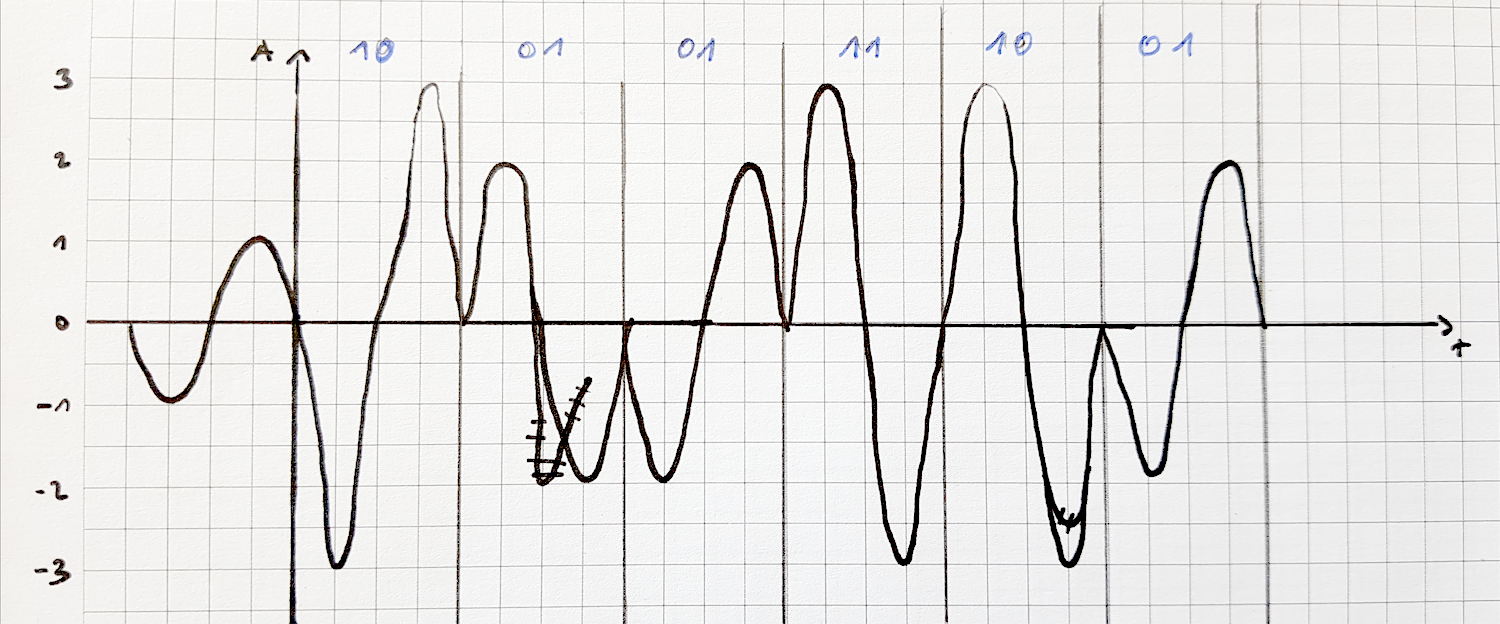
\includegraphics[width=0.9\linewidth]{modulation.png} 
	\caption{modulation diagram of bit sequence \textcolor{blue}{$[100101111001]$}.}
\end{figure}
\\
\textbf{2.  Is the modulation scheme efficient?  Explain!}\\
\\
A modulation is efficient, if it can transport many information during one Hz of transmitting. Here we only can put one Bit per Hz $\rightarrow$ not efficient.\\
\\
\textbf{3.  What is the most robust shift keying scheme?  Specify the reason!}\\
\\
The most robust scheme may be the QAM, because the bit error rate doesn't raise as high as the other schemes with increasing bit count.



\end{document}

% Hier nach passiert nichts mehr, daher nutzen wir das als kleines Cheat-Sheet ;)
% ===============================================================================

% Aufzählungen (auch merhstufig):
\begin{itemize}[itemsep=0pt]
	\item 
\end{itemize}

%Bilder eifnügen:
\begin{figure}[h!] %h! sorgt dafür dass das Bild möglichst nicht woanders hingeschoben wird
	%Erklärung: [width=0.5\linewidth] -> Bild ist maximal so breit wie die Hälfte des Schriftbildes
	\includegraphics[width=0.5\linewidth]{Bildname.jpg} 
	\caption{Bildunterschrift}
\end{figure}

%Tabelle einfügen:
\begin{table}[h!] %h! sorgt dafür dass die Tabelle möglichst nicht woanders hingeschoben wird
	\caption{Tabellenüberschrift}
	%hinter {tabular}: Anzahl Spalten (c=center, l=linksbündig, r=rechtsbündig, | Spaltenstriche)
	\begin{tabular}{|c|c|c} 
		A & B & C  \\ % \\ = return (neue zeile)
		\hline % horinzontale Linie
		0 & 1 & 2
	\end{tabular}
\end{table}
